% Chapter 4

\chapter{Processamento de Sinal} % Main chapter title
\label{chap:Chapter4} % For referencing the chapter elsewhere, use \ref{chap:Chapter4} 

%----------------------------------------------------------------------------------------

\section{Processamento de Sinal}
Como falado em \ref{contextualização}, o conceito do radar passivo é fazer uma \textit{cross-correlation} entre o sinal direto e o refletido. O problema está no facto de ser computacionalmente muito pesado fazer uma \textit{\gls{2D-CCF}}, sendo necessário a utilização de algoritmos mais eficientes para o cálculo da mesma.\par
O processamento de sinal num radar passivo pode ser, resumidamente, enumerado em oito pontos:
\begin{enumerate}
	\item Receção e reconstrução do sinal direto (\textit{reference signal}$s_{ref}$)
	\item Receção do \textit{surveillance signal} ($s_{r}$))
	\item \textit{Cross-correlation} do $s_{ref}$ e $s_{r}$
	\item Integração de produtos da correlação (FFT)
	\item Filtragem de \textit{clutter}
	\item Deteção de alvos e seguimento no domínio \textit{range/Doppler}
	\item Processamento no plano Cartesiano
	\item Seguimento no plano Cartesiano
\end{enumerate}

\subsubsection*{Equivalência entre um filtro adaptado e \textit{cross-correlation}}

Para \textit{Software Defined Radios}, a implementação de um filtro adaptado pode ser feita através do cálculo de uma \textit{cross-correlation} \parencite{Martorella}. Considerando $s_{0}(t)$ o sinal de saída do filtro adaptado e $h_{MF}(t)$ a resposta do filtro vem, 

\begin{equation} \label{4.1}
s_{0}\left( t\right) =s_{R}\left( t\right)\otimes h_{MF}\left( t\right) =\int s_{R}\left( \tau\right)s_{ref}^{\ast}\left(\tau -t\right)d\tau
\end{equation}

A equação \ref{4.1} mostra que usando um filtro adaptado obtemos um sinal de saída igual ao fazer uma \textit{cross-correlation} entre o $s_{R}$ e $s_{ref}$.\par 

Ao implementar uma \textit{cross-correlation} como mostrado em \ref{4.1}, não se toma em conta o desvio de \textit{Doppler}, visto que se faz a \textit{cross-correlation} apenas numa dimensão. Para se entrar com o desvio de \textit{Doppler} tem de se extender a \gls{2D-CCF},

\begin{equation} \label{4.2}
CCF\left( \tau,\nu\right) =\int s_{R}\left( \tau\right)s_{ref}^{\ast}\left(\tau -t\right)e^{-2\pi j\nu t}d\tau
\end{equation}

onde $\nu$ representa o desvio de \textit{Doppler} que é definido pela \textit{cross-correlation} entre o $s_{R}$ e $s_{ref}$ compensada com o \textit{Doppler shift}.\par
Como o \textit{delay-time} $\tau$ pode ser transformado em \textit{bistatic range}, a \gls{2D-CCF} pode ser representada num \textit{bistatic range-Doppler map}, através da equação \ref{4.3} que representa a \gls{2D-CCF} numéricamente visto que os sinais têm de ser digitalizados com uma certa frequência de amostragem.

\begin{equation} \label{4.3}
CCF\left(l,m\right) =\sum_{n=0}^{N-1} s_{R}\left( n\right)s_{ref}^{\ast}\left(n -l\right)e^{-2\pi j\dfrac{mn}{N}}
\end{equation}

onde $n$ representa o tempo, $l$ o \textit{delay-time}, $m$ o desvio de \textit{Doppler} e $N$ o número total de amostras que depende do \gls{CPI},

\begin{equation} \label{4.4}
N=\dfrac{CPI}{T_{s}}=CPI\cdot F_{s}
\end{equation}

\subsubsection*{Eficiência do cálculo da \gls{2D-CCF}}
De modo a ter um cálculo da \gls{2D-CCF} mais eficiente, há duas condições principais a referir:
\begin{itemize}
\item Cumprir com o teorema de \textit{Nyquist}, ou seja, garantir que a frequência de amostragem é superior ou igual à largura de banda ($F_{s}\geq B$); 
\item Ter um \gls{CPI} longo de forma a obter maior ganho de integração e consequentemente melhor relação sinal-ruído.
\end{itemize}
\par
No entanto, o cálculo de uma \gls{2D-CCF} é computacionalmente muito pesado, e isto pode ser demonstrado com um pequeno exemplo: Para uma largura de banda $B=10MHz$, um $CPI=1s$ e um número de \textit{range bins} e de \textit{doppler bins} igual a 1000 cada, implica um número de multiplicações muito elevado ($10000000\cdot 1\cdot 1000\cdot 1000=10000000000$ cálculos).\par
Para solucionar este problemas existem várias soluções numéricas, como \textit{Correlation FFT}, \textit{Direct FFT} e \textit{Batches Algorithm} \parencite{Martorella}.

\subsubsection*{\textit{Correlation FFT}}
A \textit{Correlation FFT} pode ser obtida através da equação \ref{4.3} mudando o exponencial de posição como representado na eq. \ref{4.5}, de modo a obter uma nova expressão que pode ser calculada como uma \textit{cross-correlation} a uma dimensão com uma compensação de \textit{Doppler}, ou seja, \textit{Doppler bin} ($m$), a \textit{\gls{CCF}} é a \textit{cross-correlation} entre o \textit{reference signal} $S_{ref}$ e o sinal direto com um \textit{Doppler shift}.

\begin{equation} \label{4.5}
CCF\left(l,m\right) =\sum_{n=0}^{N-1} s_{R}\left( n\right)e^{-2\pi j\dfrac{mn}{N}}s_{ref}^{\ast}\left(n -l\right)
\end{equation}

Substituindo $s_{R}\left( n\right)e^{-2\pi j\dfrac{mn}{N}}$ por $s_{R}(n,m)$ vem,

\begin{equation} \label{4.6}
CCF\left(l,m\right) =\sum_{n=0}^{N-1} s_{R}\left( n,m\right) s_{ref}^{\ast}\left(n -l\right)
\end{equation}

Com isto, e sabendo que as \textit{cross-correlations} são calculadas mais eficientemente no domínio de \textit{Fourier}, vem,

\begin{equation} \label{4.7}
CCF\left(l,m\right) = IDFT\left[ S_{R}\left( k,m\right)S_{ref}^{\ast}\left(k\right)\right] 
\end{equation}

com 

\begin{equation} \label{4.8}
S_{R}\left( k,m\right)  = DFT\left[ s_{R}\left( n,m\right) \right] 
\end{equation}

\begin{equation} \label{4.9}
S_{ref}\left( k\right)  = DFT\left[ s_{ref}\left( n\right) \right] 
\end{equation}

A \gls{DFT} da versão do sinal direto com \textit{Doppler shift} pode ser calculada apenas uma vez porque a variável $m$ apenas causa um desvio circular.
Com isto, pode-se tirar algumas conclusões \parencite{Martorella}:
\begin{itemize}
\item Apenas é necessário calcular a \textit{\gls{DFT}} de $s_{R}\left( n,m\right)$ uma vez para $m=0$, visto que para outros valores de $m$ podem ser obtidos com um desvio;
\item Em cada iteração, são calculadas N multiplicações complexas e uma \textit{\gls{IDFT}}.
\end{itemize}

Com isto, concluímos que quanto menos \textit{doppler bins} existirem em relação aos \textit{range bins}, mais eficiente será o cálculo. Este pode ser expressado através da seguinte função de complexidade:

\begin{equation} \label{4.10}
O_{CF}=2Nlog_{2}(N)+N_{f}[N+Nlog_{2}(N)]
\end{equation}

onde,
$N_{f}$: "Número de doppler bins"

\subsubsection*{\textit{Direct FFT}}
Por outro lado, a \textit{Direct FFT} é um método que, tal como a \textit{Correlation FFT} deriva da interpretação da equação \ref{4.3} mas, para cada \textit{time bin} $l$, a \textit{\gls{CCF}} é a \gls{DFT} do produto do sinal recebido com a versão conjugada com \textit{delay} do \textit{reference signal} $S_{ref}$.

\begin{equation} \label{4.11}
CCF\left(l,m\right) = DFT\left[ S_{R}\left( n\right)S_{ref}^{\ast}\left(n-l\right)\right] 
\end{equation}

Da interpretação da equação \ref{4.11} conclui-se que, para cada iteração, são calculadas N multiplicações complexas e u,a \gls{DFT}. A sua função de complexidade pode ser expressa através da expressão \ref{4.12}:


\begin{equation} \label{4.12}
O_{DF}=N_{\tau}[N+Nlog_{2}(N)]
\end{equation}

onde,
$N_{\tau}$: "Número de range bins"

Ao contrário da \textit{correlation FFT}, tal como se pode observar na função de complexidade, a eficiência deste método é dependente do $N_{\tau}$. Isto é, o número de iterações feitas neste método está diretamente relacionado com o número de \textit{range cells}: quanto maior for o número de \textit{range cells} do mapa \textit{range-Doppler}, menos eficiente é este método.\par

\begin{figure}[h]
\centering
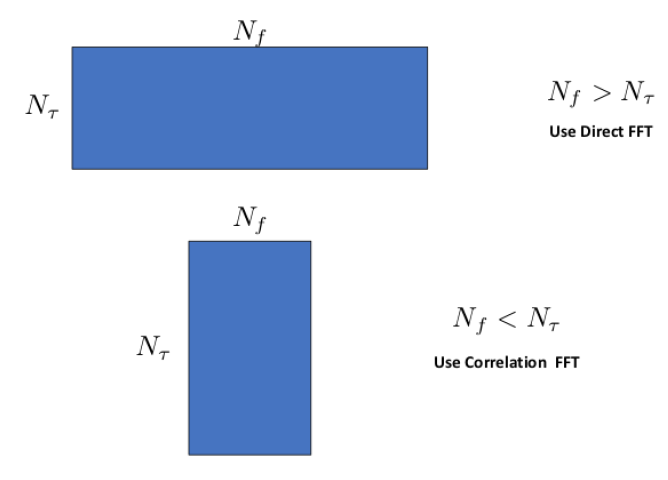
\includegraphics[scale=0.6]{chapters/ch4/assets/cfft_vs_dfft}
\caption[Correlation FFT vs Direct FFT]{\textit{Correlation FFT vs Direct FFT} (Figura 2.4 \cite{Martorella})}
\label{fig:cfft_vs_dfft}
\end{figure}

A figura \ref{fig:cfft_vs_dfft} representa de uma forma ilustrativa quando usar a \textit{Direct FFT} ou \textit{Correlation FFT} de acordo com a relação de \textit{Doppler cells} e \textit{range cells} no mapa de \textit{range-Doppler}. Se existirem mais \textit{Doppler cells} a \textit{Direct FFT} é mais eficiente, enquanto se o contrário se verificar, a \textit{Correlation FFT} torna-se mais eficiente.

\subsubsection*{\textit{Batches algorithm}}
Tanto os métodos \textit{direct FFT} e \textit{correlation FFT} são mais eficientes que fazer o cálculo da \gls{2D-CCF}, no entanto, dependem do número de \textit{range} ou \textit{doppler cells} e continuam a ser muito pesadas computacionalmente porque apenas otimizam o cálculo ao longo de uma dimensão.\par 
Apesar de não existir nenhum método perfeito que produza uma solução exata, um método denominado \textit{Batches algorithm} foi proposto e permite otimizar em duas dimensões com uma pequena perda de \textit{\gls{SNR}} reduzindo de forma considerável o peso computacional.\par
O \textit{Batches algorithm} consiste na subdivisão dos dois sinais recebidos, o sinal direto e o sinal refletido no alvo, em segmentos denominados \textit{batches}. Sendo $n_{B}$ o número de \textit{batches} e $N_{B}$ o comprimento do mesmo, com $N=n_{B}\cdot N_{B}$, a expressão da \gls{CCF} é representada pela equação \ref{4.13}.

\begin{equation} \label{4.13}
CCF\left( l,m\right)=\sum_{r=0}^{n_{B}-1}e^{\left( -j2\pi \dfrac{mrN_{B}}{N}\right)}\cdot \sum_{p=0}^{N_{B}-1}s_{R}\left( rN_{B}+p\right)s_{ref}^{\ast}\left( rN_{B}+p-l\right) e^{\left( -j2\pi \dfrac{mp}{N}\right)}   
\end{equation}

Este algoritmo assume que o efeito de \textit{Doppler} é negligenciado dentro de cada \textit{batch}, ou seja, só é calculado para o inicio de cada \textit{batch} $n_{B}$ e assim a equação \ref{4.13} é reduzida à equação \ref{4.14}.

\begin{equation} \label{4.14}
CCF\left( l,m\right)=\sum_{r=0}^{n_{B}-1}e^{\left( -j2\pi \dfrac{mrN_{B}}{N}\right)}\cdot \sum_{p=0}^{N_{B}-1}s_{R}\left( rN_{B}+p\right)s_{ref}^{\ast}\left( rN_{B}+p-l\right)
\end{equation}

A aproximação feita na eq. \ref{4.14} (frequência com que se calcula o desvio de \textit{Doppler}) pode ser representada por uma função \textit{step-wise} em vez de uma função linear (figura \ref{fig:phase_ap}).

\begin{figure}[h]
\centering
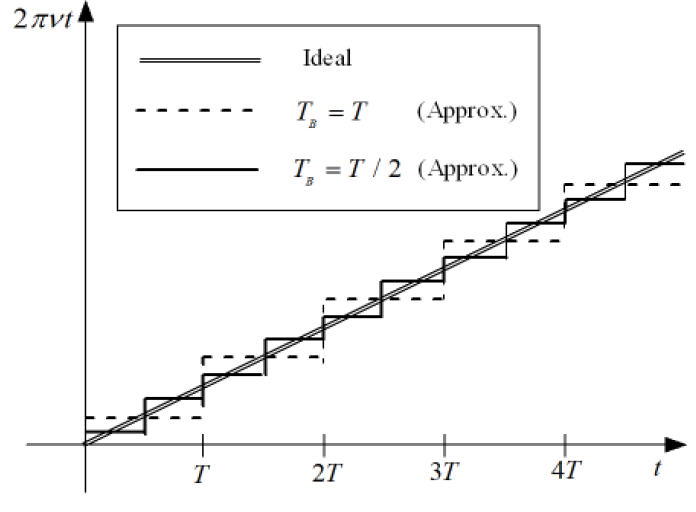
\includegraphics[scale=0.6]{chapters/ch4/assets/phase_ap}
\caption[Aproximação de fase]{Aproximação de fase da função de \textit{step} comparada com o ideal: função linear (Figura 2.6 \cite{Martorella})}
\label{fig:phase_ap}
\end{figure}

A equação \ref{4.14} pode ser interpretada de uma forma mais simples (eq. \ref{1.15})ao considerar o somatório do produto entre $s_{R}$ e $s_{R^{\ast}}$ como uma \gls{CCF} e a cada $n_{B}$ é calculado a \gls{DFT} ao longo de $r$.

\begin{equation} \label{4.15}
CCF\left( l,m\right)=\sum_{r=0}^{n_{B}-1}CCF\left( l,r\right) e^{\left( -j2\pi \dfrac{mrN_{B}}{N}\right)}=DFT\left[ CCF\left( l,r\right) \right] 
\end{equation}

Um dos fatores que influencia a eficiência do algoritmo é a escolha da duração dos \textit{batches}. Com isto, é simples concluir que para um determinado intervalo, ao escolher \textit{batches} com maior duração, vai existir um menor número de \textit{batches}, e consequentemente, a \gls{DFT} é calculada ao longo de um menor número de pontos o que vai levar a um menor tempo de processamento. No entanto, ao escolher \textit{batches} com maior duração, vai introduzir um erro maior na aproximação de fase e consequentemente mais perdas em \gls{SNR}.\par
Contudo, \textit{batches} com menor duração implicam o contrário, ou seja, maior número de batches, maior tempo de processamento e menos perdas em \gls{SNR}. \par 
Foi desenvolvido um estudo de grande interesse \parencite{Petri2012} que analisa extensivamente a utilização do \textit{batches algorithm} em que foram recolhidos dados com um radar passivo da \gls{CNIT}. Os resultados da análise da duração dos \textit{batches} com o tempo de processamento e perdas \gls{SNR} encontram-se representados na tabela e figura \ref{fig:bat_snr} respetivamente.\par 

\begin{table}[h]
\centering
\begin{tabular}{@{}ccccc@{}}
\toprule
Comprimento do batch & Tempo de processamento  \\ \midrule
31.28 $\mu s$        & 4.93 $s$                \\
218.76 $\mu s$       & 0.92 $s$                \\
333.29 $\mu s$       & 0.71 $s$                \\ 
924 $\mu s$          & 0.59 $s$                \\ \bottomrule
\label{tab:Tempo de processamento}
\end{tabular}
\caption[\textit{Batches algorithm} - tempo de processamento]{\textit{Batches algorithm} - Análise do tempo de processamento devido ao comprimento dos \textit{batches} (Tabela 2.1 \cite{Martorella})}
\end{table}

\begin{figure}[h]
\centering
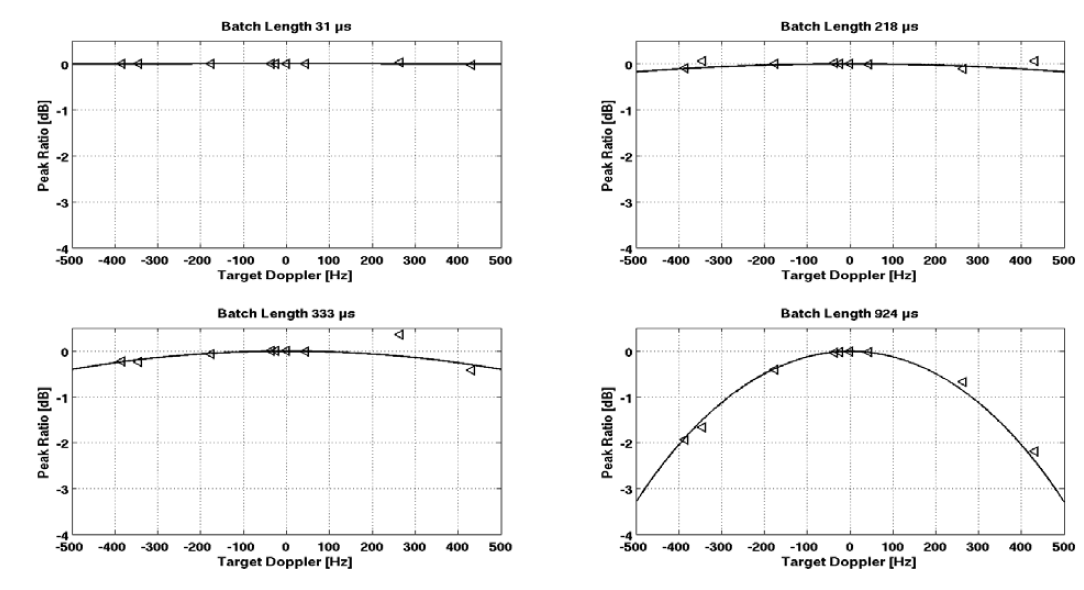
\includegraphics[scale=0.5]{chapters/ch4/assets/bat_snr}
\caption[Perdas SNR]{\textit{Batches algorithm} - Análise perdas \gls{SNR} devido ao comprimento dos \textit{batches}(Figura 2.8 \cite{Martorella})}
\label{fig:bat_snr}
\end{figure}



\subsection{Cancelamento de \textit{clutter}}
No funcionamento do radar passivo, um dos sinais que se quer ter conhecimento é o sinal direto, que é o sinal que é transmitido diretamente do iluminador de oportunidade para o recetor, como representado na figura \ref{fig:esquema_pcl}. Este sinal é submetido a uma atenuação  %de $1/C^{2}$ \parencite{Griffiths2017}, onde $C$ é a \textit{baseline} representada na figura \ref{fig:geom}.
pequena relativamente ao sinal refletido, isto porque a \textit{baseline} $C$ representada na figura \ref{fig:geom} é sempre menor que o \textit{bistatic range}. Logo, o sinal direto pode ser muito mais forte comparado com os ecos dos alvos, o que dificulta a deteção de alvos.\par 

\begin{figure}[h]
\centering
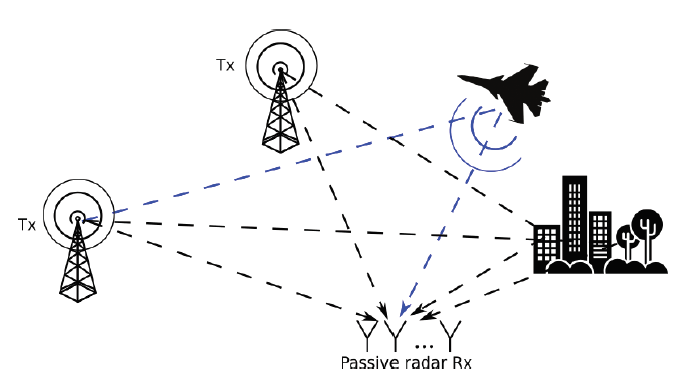
\includegraphics[scale=0.6]{chapters/ch4/assets/clutter}
\caption[Cenário PCL - Clutter]{Cenário PCL - Clutter (Figura 1 \cite{Peto2018})}
\label{fig:clutter}
\end{figure}


Por mais que se tente fisicamente não receber o sinal direto na antena de \textit{surveillance}, este e todas as suas cópias atrasadas no tempo devido a reflexões em objetos e terreno não desejadas (\textit{clutter} representado na figura \ref{fig:clutter}) são mais fortes que o sinal refletido no alvo. É possível haver reflexões em edifícios ou algo perto da antena de \textit{surveillance} que possam ser confundidas com o sinal que pretendemos obter, o que pode complicar o cancelamento de todas as réplicas do sinal indesejadas. É de notar, que no caso dos radar \textit{\gls{PCL}}, ou seja, radares passivos, estamos perante uma geometria bistática e isto leva a que o nível de \textit{clutter} na zona da \textit{baseline} possa ser muito forte e ser notável em algumas \textit{range cells}. Este efeito em junção com o sinal direto que possa ser captado na antena de \textit{surveillance} podem dificultar a deteção de alvos.\par 
O sinal recebido pode ser interpretado de uma forma mais realista como na equação \ref{4.16} para facilitar os processos de cancelamento de \textit{clutter} e identificação das diferentes componentes do sinal.


\begin{equation} \label{4.16}
S_{R}=A_{R}s_{T}\left( t\right)+\sum_{m=1}^{N_{T}}a_{m}s_{T}\left( t-\tau_{T_{m}}\right)e^{\left( 2\pi j f_{D_{m}}t\right)}+\sum_{i=1}^{N_{s}}b_{i}s_{T}\left( t-\tau_{c_{i}}\right)+n\left( t\right)    
\end{equation}

Onde o primeiro termo representa a componente do sinal direto, o segundo termo representa o sinal refletido no alvo, o terceiro termo representa o \textit{clutter} e por fim, o quarto termo representa a componente de ruído.\par

Os aspetos mais importantes na \textit{performance} do cancelamento de \textit{clutter} são a capacidade de operação em tempo real e a eficiência do algoritmo representada no mapa \textit{range-Doppler}. De modo geral, a filtragem, ou cancelamento de \textit{clutter} é feita em dois domínios diferentes: Técnicas de supressão no domínio do espaço para lidar com interferências de alta potência e algoritmos de filtragem de \textit{clutter} no domínio do tempo. Tem sido investigado a aplicação de vários métodos e o artigo \cite{Peto2018} resume a aplicabilidade e comparação de resultados obtidos na utilização dos mesmos tanto como uma explicação sucinta na sua execução.\par 

Existem várias técnicas de cancelamento de \textit{clutter} utilizadas em radares passivos. Os algoritmos de filtragem no domínio do tempo utilizam o \textit{reference signal} de modo a cancelar as réplicas do sinal com um desvio no tempo e de \textit{Doppler} no canal de \textit{surveillance}. Entre estes podemos salientar a aplicação das técnicas de filtragem de \textit{Wiener} com \textit{sample matrix inversion}, \gls{ECA}, \gls{ECA-B}, \gls{ECA-S} \gls{SCA}, \gls{LMS}, \gls{NLMS} e \gls{RLS}.\par

Como jeito de conclusão deste tópico, as figuras \ref{fig:doppler_cancelationtec} e \ref{fig:comp_cost}, retiradas do estudo \cite{Petri2012}  representam a \textit{performance} dos 
vários algoritmos nos dois aspetos mais relevantes, respetivamente no mapa de \textit{range-Doppler} que permite a observação da distorção e resolução do algoritmo e do aumento de \gls{SINR} em relação ao custo computacional  medido em \gls{FLOPS}.


\begin{figure}[h]
\centering
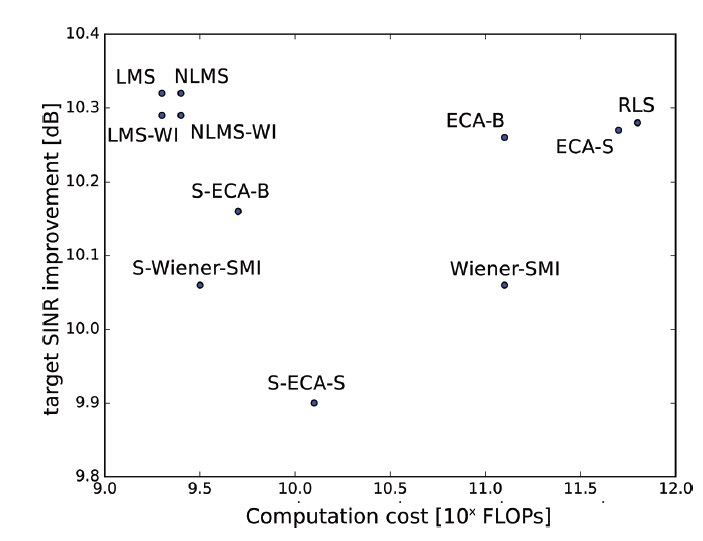
\includegraphics[scale=0.5]{chapters/ch4/assets/comp_cost}
\caption[Mapa da performance dos algoritmos]{Mapa da \textit{performance} dos algoritmos de acordo com o aumento de \gls{SINR} e \textit{computation cost} em \gls{FLOPS} (Figura 16 \cite{Peto2018})}
\label{fig:comp_cost}
\end{figure}

\begin{figure}[h]
\centering
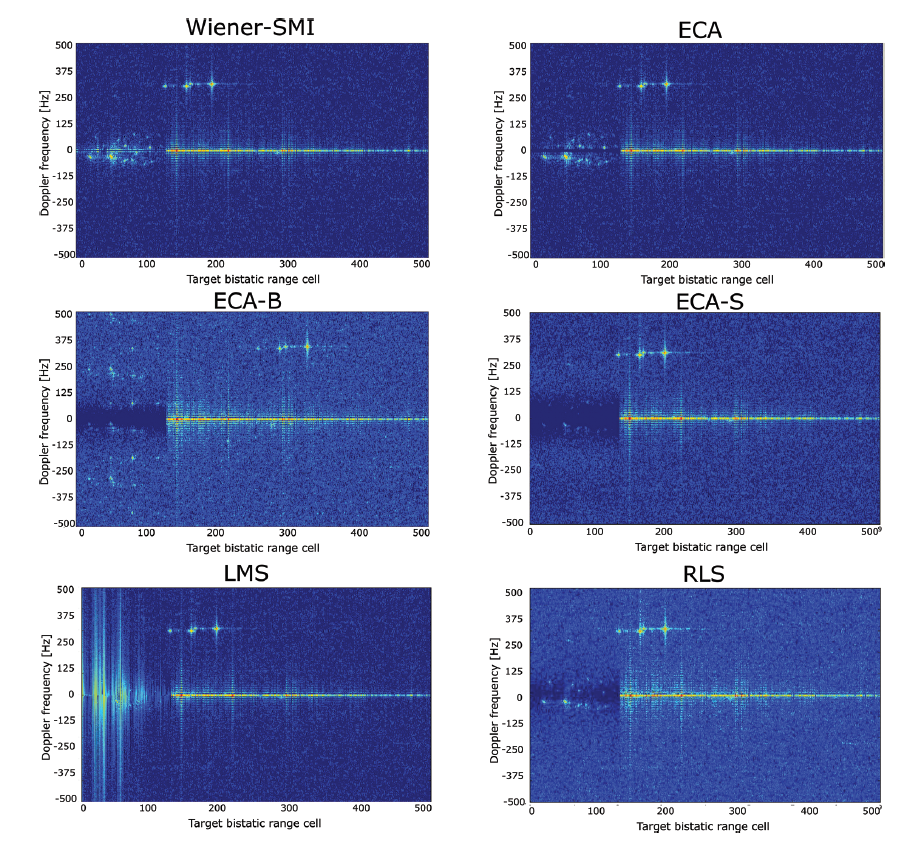
\includegraphics[scale=0.5]{chapters/ch4/assets/doppler_cancelationtec}
\caption[Mapas de range-Doppler dos diferentes algoritmos utilizados]{Mapas de \textit{range-Doppler} dos diferentes algoritmos utilizados (Figura 14 \cite{Peto2018})}
\label{fig:doppler_cancelationtec}
\end{figure}


Destes resultados obtidos, é de realçar o algoritmo \gls{ECA-S} que obteve a melhor \textit{performance} ao custo de um grande \textit{computation cost}. Contudo, pode-se observar os algoritmos do tipo \gls{LMS} e \gls{NLMS}, que apesar de terem um bom aumento de \gls{SINR} com pouco custo computacional, apresentam, como observável na figura \ref{fig:doppler_cancelationtec}, uma grande distorção no mapa \textit{range-Doppler}. Também é de notar, que na figura \ref{fig:comp_cost}, o aumento de \gls{SINR} é pouco relativamente ao custo computacional, isto porque o referencial não está normalizado, ou seja, a janela do eixo das ordenadas toma valores entre $9.8$ e $10.4 dB$ enquanto a janela do eixo das abcissas toma valores entre $10^{9}$ e $10^{12} FLOPS$.


\subsection{Reconstrução e equalização do sinal direto}
Uma das principais diferenças do radar passivo para o radar ativo é que no último o \textit{reference signal} é conhecido visto que é transmitido pelo próprio radar. No caso do radar passivo, a utilização de iluminadores de oportunidade tem como consequências o não conhecimento do sinal direto, visto que para além de receber o mesmo, recebemos as suas réplicas atrasadas no tempo e em \textit{Doppler} e ainda ruído.\par 
De forma a melhorar o sinal direto em quando este é digital, neste subcapítulo vão ser discutidos dois métodos diferentes para a remoção de \textit{multipath} e remoção de picos espúrios formados na função de ambiguidade.

\subsubsection*{Reconstrução do sinal direto} \label{Reconstrução do sinal direto}
Alguns sinais digitais transmitidos, como \gls{DVB-T} em específico, permitem a reconstrução do sinal direto através da desmodulação e re-modulação do sinal direto recebido. Por forma a reconstruir o sinal direto, no caso da \gls{DVB-T}, é importante conhecer o comprimento do símbolo exprimido em amostras, isto porque se a frequência de amostragem do transmissor e do recetor for igual, o comprimento do sinal em amostras é inteiro e a sua receção consiste em meter o sinal no domínio da frequência, usando uma \gls{FFT}. Se este não for o caso, ou seja, que a frequência de amostragem do recetor não seja a definida pelo \textit{standard} \gls{DVB-T}, o comprimento do símbolo não vai ser um número inteiro e a constelação do sinal recebido vai ficar distorcida visto que os pontos depois de usar a \gls{FFT} não vão corresponder às posições de cada subportadora. As soluções para este problema podiam passar por fazer uma nova amostragem do sinal por interpolação, mas isso ia introduzir grandes distorções. Existem várias soluções para este problema, como a utilização de outras transformadas, como a \gls{CZT}.\par 
O próximo passo na receção do sinal \gls{DVB-T} é descodificar os símbolos \gls{OFDM}. Este processo passa por o cálculo inverso no espetro do sinal que foi realizado no transmissor, ou seja, se foi usado uma \gls{FFT} no transmissor, para descodfidicar os símbolos \gls{OFDM} usa-se uma \gls{IFFT}. É de notar que, como falado no parágrafo anterior, se a frequência de amostragem for diferente no transmissor e recetor, a \gls{FFT} que é o mais comum, não pode ser usada. Ao invés, usa-se um método baseado na \gls{CZT}, que não é abordado nesta dissertação, mas pode ser compreendido, tal como todo o processo de reconstrução do sinal direto para radares passivos no estudo \cite{Baczyk2011}.\par 
De seguida, tem-se uma constelação do sinal direto reconstruido como na figura \ref{fig:64QAM} e o próximo passo é a reprodução do sinal no domínio do tempo sem o efeito de \textit{multipath}.

\begin{figure}[h]
\centering
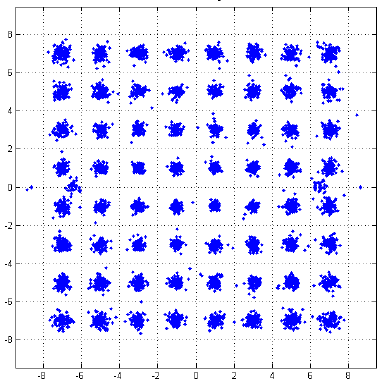
\includegraphics[scale=0.7]{chapters/ch4/assets/64QAM}
\caption[Constelação 64QAM]{Constelação 64QAM (Figura 3.4 \cite{Martorella})}
\label{fig:64QAM}
\end{figure}


\subsubsection*{Equalização do sinal direto}
Em adição à remoção do efeito \textit{multipath} com a reconstrução do sinal direto, é possível equalizar o sinal de forma a remover picos espúrios formados na função de ambiguidade como representados na figura \ref{fig:ACF} relativamente a sinais \gls{DVB-T}.

\begin{figure}[h]
\centering
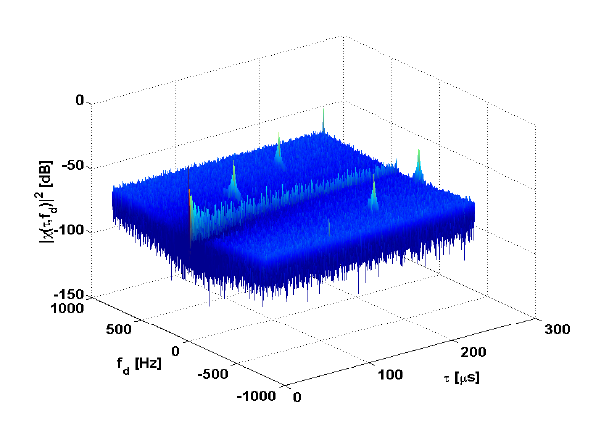
\includegraphics[scale=0.7]{chapters/ch4/assets/ACF}
\caption[Função de ambiguidade - Sinal DVB-T]{Função de ambiguidade - Sinal DVB-T - Presença de picos espúrios (Figura 3.5 \cite{Martorella})}
\label{fig:ACF}
\end{figure}

Um algoritmo eficiente para remover estes picos espúrios passa por estimar tanto para o sinal direto $S_{ref}$ como para um sinal, neste caso \gls{DVB-T}, gerado localmente uma função de \textit{\gls{PSD}} e, equalizar através de uma função de filtragem $H$ que posteriormente, é multiplicada com a transformada do sinal direto $S_{ref}$. De seguida é aplicada a \gls{IFFT} de forma a gerar um sinal direto mais limpo. Um esquema de blocos do algoritmo está representado na figura \ref{fig:equal}.

\begin{figure}[h]
\centering
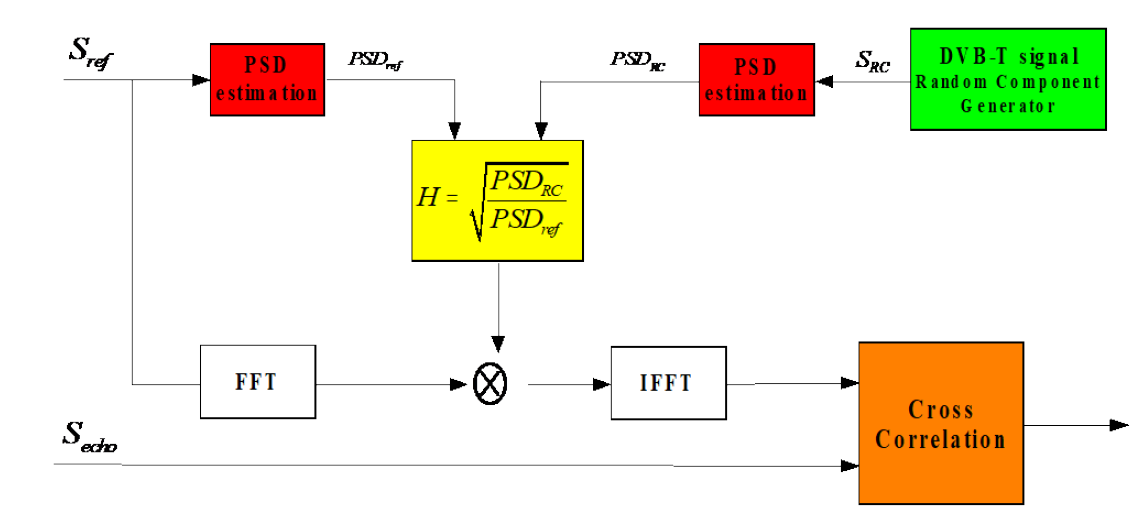
\includegraphics[scale=0.5]{chapters/ch4/assets/equal}
\caption[Diagrama de blocos - Algoritmo de equalização]{Diagrama de blocos - Algoritmo de equalização(Figura 3.6 \cite{Martorella})}
\label{fig:equal}
\end{figure}



\section{Simulação}

\subsection{Função de Ambiguidade}
Uma ferramenta que permite analisar as propriedades do sinal utilizado como iluminador de oportunidade é a função de ambiguidade. Esta função é bidimensional no \textit{time-delay} e em \textit{Doppler}, que representa a distorção devido ao filtro adaptado do recetor, falado no inicio deste capítulo e às propriedades do sinal.\par 
Para um sinal $s(t)$, a sua função de ambiguidade é obtida pela equação \ref{4.17}.

\begin{equation} \label{4.17}
\chi\left( \tau,f\right) =\int s\left( t\right)s^{\ast}\left( t-\tau\right)e^{2\pi jft}dt
\end{equation}

, ou seja, a auto-correlação do sinal recebido.

Utilizando o \textit{matlab} e as ferramentas que este dispõe, é possível calcular funções de ambiguidade de diversos sinais, tendo como um exemplo a figura \ref{fig:ambfun_fmdef} que é resultado do código em anexo \ref{Annex1} apresentado pelo matlab para fazer funções de ambiguidade consoante as caraterísticas do sinal.
\begin{figure}[h]
\centering
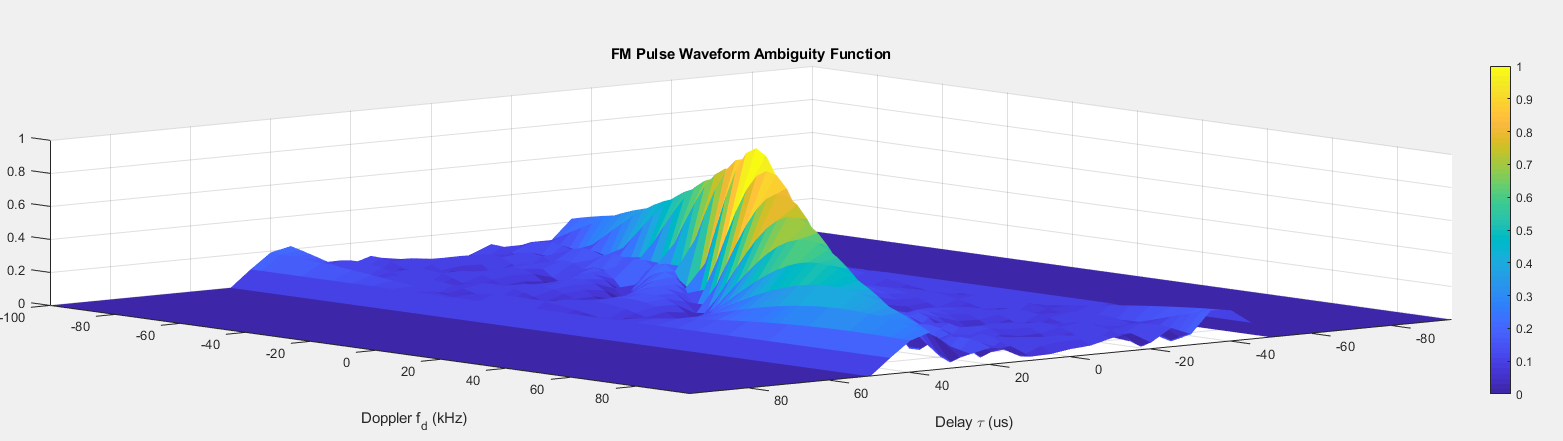
\includegraphics[scale=0.4]{chapters/ch4/assets/ambfun_fmdef}
\caption[Função de ambiguidade para um pulso FM]{Função de ambiguidade para um pulso FM}
\label{fig:ambfun_fmdef}
\end{figure}


\subsubsection{Sinais FM}
Um dos fatores que influencia a performance do sistema é a largura de banda, o que no caso de sinais \gls{FM} é dependente do tipo de música que é transmitido.\par
A figura \ref{fig:ambfun2} é retirada de uma estação a transmitir notícias que corresponde aos gráficos de cima e a transmitir música pop, representado no gráfico de baixo. As principais conclusões que se podem retirar da análise da função de ambiguidade de ambas é que quando é transmitida música, especialmente estilos de músicas como \textit{hard rock}, a largura de banda do sinal transmitido aumenta o que provoca uma função mais estreita e com menor intensidade em redor dos planos de zero \textit{Doppler} e zero \textit{delay}. Consequentemente, este tipo de transmissões permitem uma melhor deteção não só em alcance, como em \textit{Doppler}.

\begin{figure}[h]
\centering
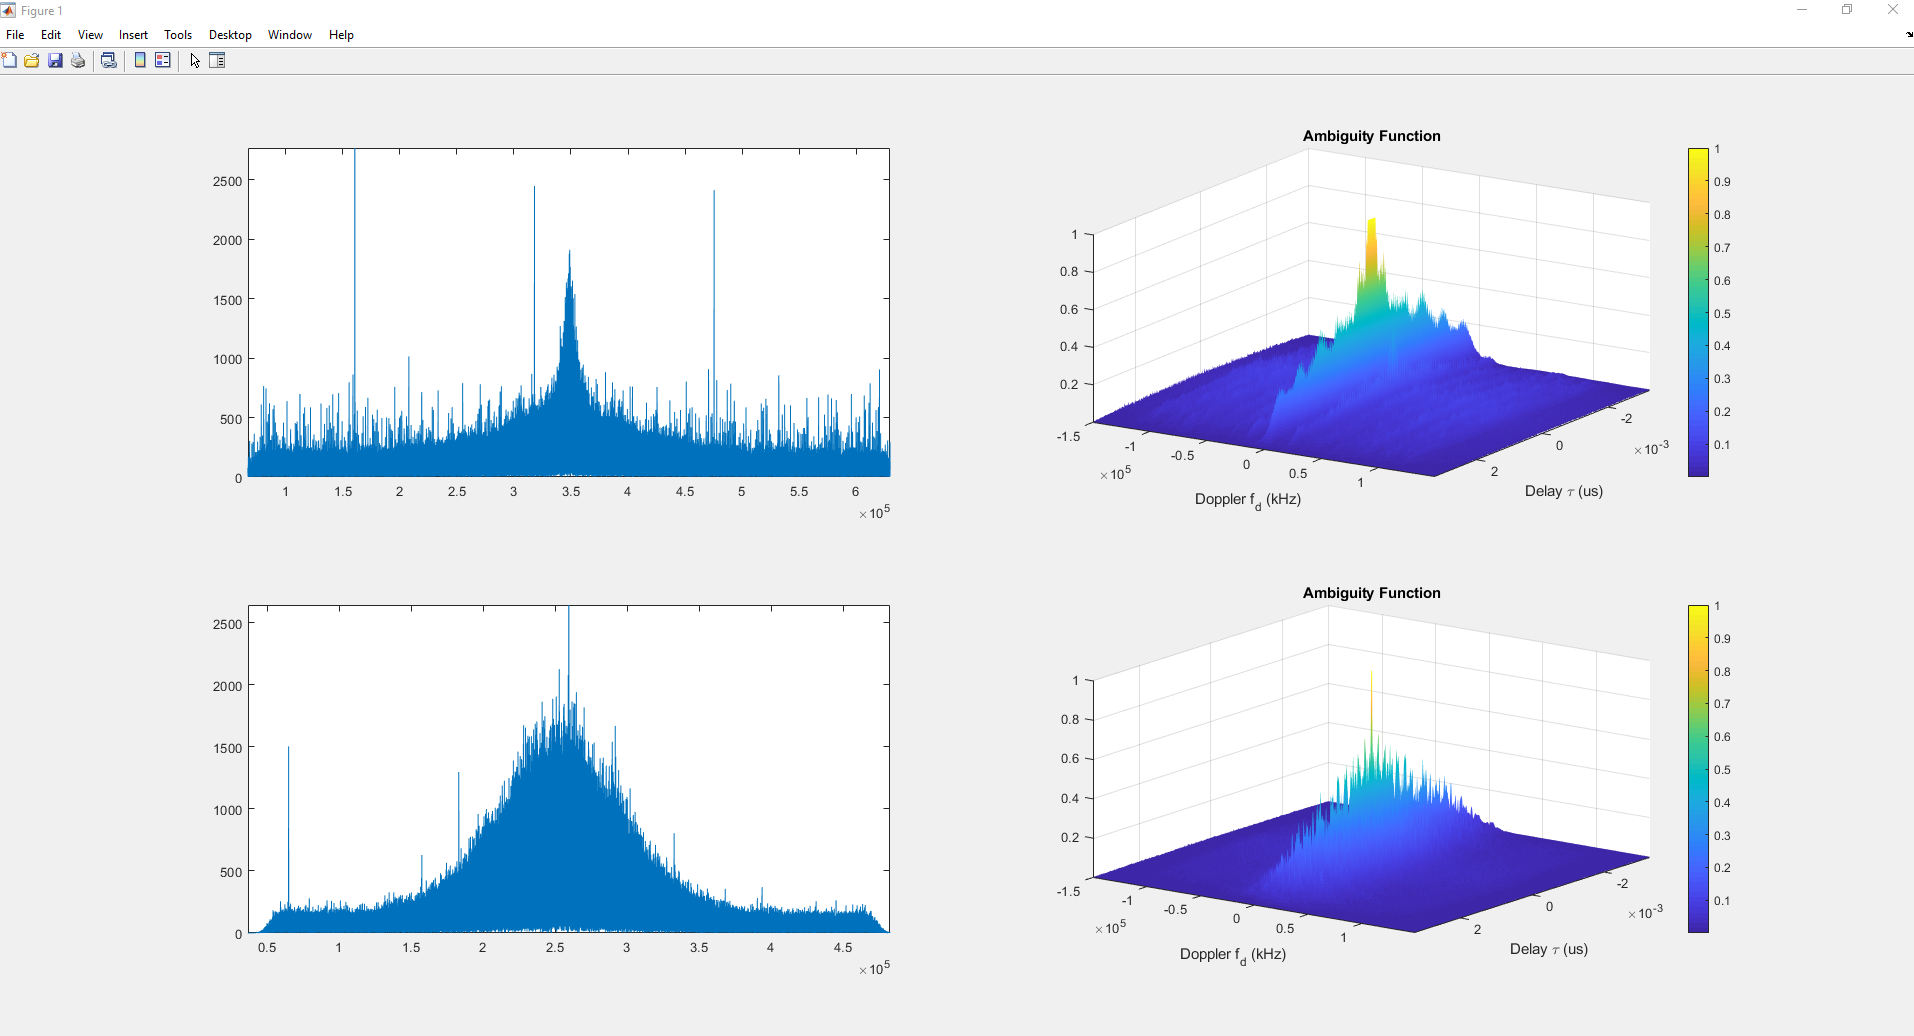
\includegraphics[scale=0.3]{chapters/ch4/assets/ambfun2}
\caption[Função de ambiguidade para uma estação FM]{Função de ambiguidade para um pulso FM retirada de uma estação a dar notícias e música pop}
\label{fig:ambfun2}
\end{figure}
 


\subsubsection{Sinais DVB-T}
Para obter as funções de ambiguidade dos sinais \gls{DVB-T} foi utilizado o LimeSDR com duas antenas de $24 dB$, como descrito no Capítulo \ref{chap:Chapter6}. É de notar que que a antena utilizada no lado direito tem um ganho relativamente superior, o que se deve às fichas que foram cravadas, mas que não tem muito impacto na função de ambiguidade. Dito isto, é mais adequado utilizar este canal para o sinal refletido e o com menor ganho para o sinal direto.\par 

\begin{figure}[h]
\centering
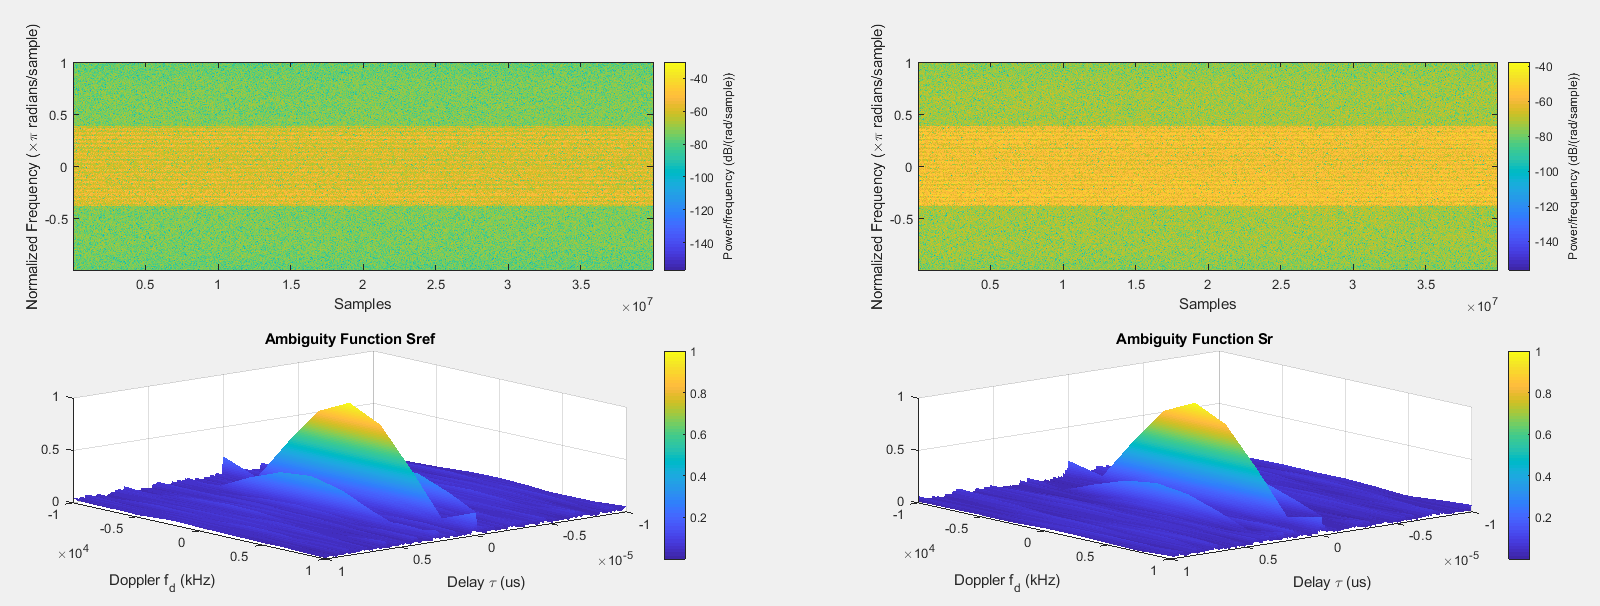
\includegraphics[scale=0.35]{chapters/ch4/assets/dvbt}
\caption[Função de ambiguidade para dois sinais DVB-T]{Função de ambiguidade para dois sinais DVB-T}
\label{fig:dvbt}
\end{figure}
 
Através da equação \ref{4.18}, na frequência $f_{0}=602 MHz$ que é utilizada nesta zona para \gls{DVB-T}, com $c=3x10^{8}m/s$, obtém-se um valor de de variação de frequência de $100Hz$ para $50m/s=180km/h$, ou seja, para uma distância ao alvo com valores inferiores a $15m$, segundo a equação \ref{4.19} para um \textit{delay} de $1\times 10^{-7}$, é muito difícil a deteção da velocidade do alvo.

\begin{equation} \label{4.18}
\Delta f=\dfrac{\Delta v}{c}f_{0}
\end{equation}

\begin{equation} \label{4.19}
Range=\dfrac{c\times delay}{2}
\end{equation}


